\section{Number Systems} 

\subsection{Natural Numbers}

  Note that the axiom of infinity allows us to construct the ordinal numbers. This was based off of two things. First the assertion that the empty set is contained and that if a set $w$ in the ordinal numbers, then $w \cup \{w\}$ is also contained. The second property has a name. 

  \begin{definition}[Inductive Set] 
    Let $X$ be a set. Then $X$ is said to be \textbf{inductive} if every element has a \textbf{successor}, i.e. a construction of a different element $y$ from $x$.  
    \begin{equation}
      x \in X \implies f(x) \in X
    \end{equation}
    A set 
    $X \subset \mathbb{R}$ is inductive if for each number $x \in X$, it also contains $x + 1$. 
  \end{definition} 

  From this, with a few more structures we can define the naturals. 

  \begin{definition}[Natural Numbers]
    The natural numbers $\mathbb{N}$ is the set of von Neumann ordinals, with each element represented by a numerical symbol (e.g. $1, 2, \ldots$). 
    \begin{align*}
      0 & = \{\} = \emptyset \\
      1 & = \{0\} = \{\emptyset\} \\
      2 & = \{0,1\} = \{\emptyset,\{\emptyset\}\} \\
      3 & = \{0,1,2\} = \{\emptyset,\{\emptyset\},\{\emptyset,\{\emptyset\}\}\} \\
      4 & = \{0,1,2,3\} = \{\emptyset,\{\emptyset\},\{\emptyset,\{\emptyset\}\},\{\emptyset,\{\emptyset\},\{\emptyset,\{\emptyset\}\}\}\} \\
      \ldots & = \ldots 
    \end{align*} 
    The successor function $S(x)$ is rewritten in different notation as $S(x) = x + 1$. It also has the relation $\leq$ defined as the set
    \begin{equation}
      \{ (a, b) \in \mathbb{N} \times \mathbb{N} \mid \exists n (S^n(a) = b )\}
    \end{equation}
    where $S^n$ is the successor operation composed $n$ times. Addition is defined as 
    \begin{equation}
      a + b \coloneqq S^b (a) = S^a (b)
    \end{equation}
    and multiplication is defined recursively as 
    \begin{enumerate}
      \item $m \times 0 \coloneqq 0$. 
      \item $m \times (n + 1) \coloneqq m \times n + m$
    \end{enumerate}
    which is familiar to the process of adding $m$ to itself $n$ times. 
  \end{definition}

  \begin{lemma}[Well Ordering Principle of Naturals]
    Every nonempty subset of $\mathbb{N}$ has a minimal element. 
  \end{lemma} 
  \begin{proof}
    Take a subset $A \subset \mathbb{N}$. 
    \begin{enumerate}
      \item If $0 \in A$, the minimum is $0$. 
      \item Else if $1 \in A$, the minimum is $1$. 
      \item ...
    \end{enumerate} 
  \end{proof}

  We can use this inductive property of natural numbers to prove properties of them. Note that this can only be used to prove for finite (yet unbounded) numbers! 

  \begin{lemma}[Induction Principle]
    Given $P(n)$, a property depending on a natural number $n \in \mathbb{N}$, 
    \begin{enumerate}
      \item if $P(n_0)$ is true for some $n_0 \in \mathbb{N}$, and
      \item if for every $k \geq n_0$, $P(k)$ true implies $P(k+1)$ true, 
    \end{enumerate}
    then $P(n)$ is true for all $n \geq n_0$. 
  \end{lemma}

  \begin{lemma}[Strong Induction Principle]
    Given $P(n)$, a property depending on a positive integer $n$, 
    \begin{enumerate}
      \item if $P(n_0), P(n_0 + 1), \ldots, P(n_0 + m)$ are true for some positive integer $n_0$, and nonnegative integer $m$, and 
      \item if for every $k > n_0 + m, P(j)$ is true for all $n_0 \leq j \leq k$ implies $P(k)$ is true, 
    \end{enumerate}
    then $P(n)$ is true for all $n \geq n_0$. 
  \end{lemma} 

  \begin{theorem}[Equivalence of 3 Principles]
    The well-ordering principle, induction principle, and the strong induction principle are all equivalent. 
  \end{theorem}
  \begin{proof}
    We prove the steps. 
    \begin{enumerate}
      \item \textit{Well Ordering $\implies$ Strong Induction}. 
      \item \textit{Strong Induction $\implies$ Induction}.  
      \item \textit{Induction $\implies$ Well-Ordering}. 
    \end{enumerate}
  \end{proof}

  The idea behind the strong induction principle leads to the proof using infinite descent. Infinite descent combines strong induction with the fact that every subset of the positive integers has a smallest element, i.e. there is no strictly decreasing infinite sequence of positive integers. 

  \begin{theorem}[Infinite Descent]
    Given $P(n)$, a property depending on positive integer, assume that $P(n)$ is false for a set of integers $\mathcal{S}$. Let the smallest element of $\mathcal{S}$ be $n_0$. If $P(n_0)$ false implies $P(k)$ false, where $k < n_0$, then by contradiction $P(n)$ is true for all $n$. 
  \end{theorem}

\subsection{Integers} 

  \begin{theorem}[Countability]
    $\mathbb{Z}$ is countable. 
  \end{theorem}

\subsection{Rational Numbers} 

  \begin{theorem}[Rational Numbers]
    $\mathbb{Q}$ is countable. 
  \end{theorem}
  \begin{proof}
    Since $\mathbb{N} \approx \mathbb{Z}$, it suffices to prove that $\mathbb{N} \times \mathbb{N}$ is countable. We wish to find the bijection $f: \mathbb{N} \times \mathbb{N} \rightarrow \mathbb{N}$. We claim that 
    \begin{equation}
      f(x, y) = \frac{1}{2} \big\{ (x + y - 1)^2 - (x + y - 1) + 2 \big\} + x - 1
    \end{equation}
    \begin{figure}[H]
      \centering 
      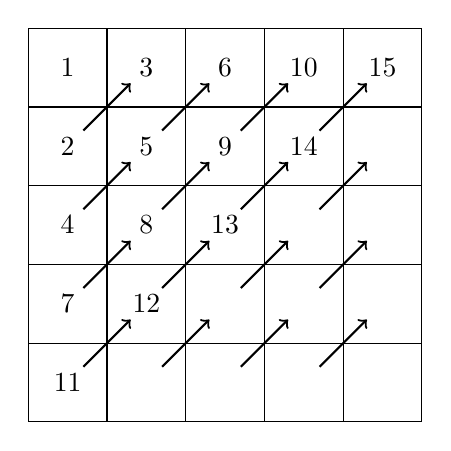
\begin{tikzpicture}[scale=1]
        % Grid
        \draw (0,0) grid (5,5);
        
        % Numbers specified (top-right triangle)
        \node at (0.5,4.5) {1};
        \node at (1.5,4.5) {3};
        \node at (2.5,4.5) {6};
        \node at (3.5,4.5) {10};
        \node at (4.5,4.5) {15};
        
        \node at (0.5,3.5) {2};
        \node at (1.5,3.5) {5};
        \node at (2.5,3.5) {9};
        \node at (3.5,3.5) {14};
        
        \node at (0.5,2.5) {4};
        \node at (1.5,2.5) {8};
        \node at (2.5,2.5) {13};
        
        \node at (0.5,1.5) {7};
        \node at (1.5,1.5) {12};
        
        \node at (0.5,0.5) {11};
        
        % Diagonal arrows
        \foreach \x in {0,...,3} {
            \foreach \y in {0,...,3} {
                \draw[->, thick] (\x+0.7,\y+0.7) -- (\x+1.3,\y+1.3);
            }
        }
      \end{tikzpicture}
      \caption{You can see that given $(x, y)$ it is on the $(x+y+1)$th diagonal, which starts from the $\frac{1}{2} \big((x+y+1)^2 - (x+y+1) + 2)$th number and increments by $x-1$. Therefore, we have the formula above. } 
      \label{fig:rationals_countable}
    \end{figure}
  \end{proof}

\subsection{Real Numbers} 

  The construction of the real numbers is done in my real analysis notes. We will prove the uncountability of the reals assuming you know the construction. 

  \begin{theorem}[Uncountability of Infinite Binary Numbers]
    Let $A$ be the set of all sequences whose elements are the digits $0$ and $1$. Then, $A$ is uncountable. 
  \end{theorem}

  We also know that $\mathbb{R}$ is equipotent to $A$, and so the corollary follows. 

  \begin{corollary}[Uncountability of Reals]
    $\mathbb{R}$ is uncountable. 
  \end{corollary}

\subsection{Exercises} 

  \begin{exercise}[Math 531 Spring 2025, PS1.1]
    Find a formula for the sum of the first $n$ odd numbers and prove that it is correct.
  \end{exercise}
  \begin{solution}
    I claim that $f(n) = n^2$. I prove using induction. For $n = 1$, $f(1) = n^2 = 1^2 = 1$. Now assume $f$ holds for some $k \in \mathbb{N}$. Then, the $k$th off number is $2k-1$. Therefore 
    \begin{equation}
      f(k+1) = f(k) + (2k + 1) = k^2 + 2k + 1 = (k + 1)^2
    \end{equation}
    and the formula holds for $k=1$. By the principle of induction, $f(n) = n^2$ is true for all $n \in \mathbb{N}$. 
  \end{solution}

  \begin{exercise}[Shifrin Abstract Algebra 1.1.4.C]
    We check for $n = 1$ denoting our formula as $f$. Indeed, we have 
    \begin{equation}
      f(1) = \frac{1 \cdot 2 \cdot 3}{6} = 1 = 1^2
    \end{equation} 
    For the induction step, assume that $f(k)$ is true for some $k \in \mathbb{N}$. Then, 
    \begin{align}
      f(k+1) & = f(k) + (k+1)^2 \\
             & = \frac{k (k + 1) (2k + 1)}{6} + \frac{6 (k+1)^2}{6} \\
             & = \frac{(k+1) \{ k (2k+1) + 6(k+1)\}}{6} \\
             & = \frac{(k+1) (2k^2 + 7k + 6)}{6} \\
             & = \frac{(k+1)(k+2)(2(k+1) + 1)}{6} \\
             & = f(k+1)
    \end{align}
    Therefore $f$ holds for all $n \in \mathbb{N}$. 
  \end{exercise} 

  \begin{exercise}[Shifrin Abstract Algebra 1.1.4.G]
    We prove the base cases for $n = 1, 2, 3$. 
    \begin{enumerate}
      \item $n = 1$. $n+2 = 3$ is divisible by $3$. 
      \item $n = 2$. $n+4 = 6$ is divisible by $3$. 
      \item $n = 3$. $n+2 = 3$ is divisible by $3$. 
    \end{enumerate} 
    For our inductive step, assume that for some $n = k \in \mathbb{N}$, one of the elements in $S_k = \{k, k+2, k+4\}$ is divisible by $3$. Let us denote this element $a$. We wish to show that this claim is true for $n = k+3$ on the set $S_{k+3} = \{k+3, k+5, k+7\}$. Since $a \in S_k$, this means that $a+3 \in S_{k+3}$, and $3 | a \implies 3 | (a+3)$. So we can always identify the element $a+3$. Since we proved the base cases for $n=1, 2, 3$, and proved the recursive step, we have essentially proved the claim for all naturals of the form $3k+1, 3k+3, 3k+3$ ($k \in \mathbb{N}_0$), which is precisely the natural numbers. 
  \end{exercise}

  \begin{exercise}[Shifrin Abstract Algebra 1.1.4.J]
    Let $n = 1$. Then $1 + x \geq 1 + x$ trivially. For the induction step, assume that this inequality holds for some $n \in \mathbb{N}$. Then, we have 
    \begin{align}
      1 + (n+1) x & = 1 + nx + x \\
                  & \leq (1+x)^n + x \\ 
                  & \leq (1+x)^n + x(1+x)^n \\
                  & = (1+x)^{n+1}
    \end{align} 
    where the prove the penultimate step by applying the ordered field axioms to the 2 cases: 
    \begin{enumerate}
      \item If $x \geq 0$, then addition preserves order so $1 + x \geq 0 + 1 = 1$. Since $1 + x, 1 > 0$, order is preserved under multiplication by a positive element, so $(1+x)^2 \geq 1+x \geq 1$. Using induction, we can show that for all $n \in \mathbb{N}$, $(1+x)^n \geq 1$, and again by preservation of order under multiplication by a positive element, this implies $x (1 + x)^n \geq x$ for all $n \in \mathbb{N}$. 
      \item If $0 > x > -1$, we have $0 < 1 + x < 1$ and by the same induction proof, we can bound $0 < (1+x)^n < 1$ for all $n$. Finally by reversal of order under multiplication by a negative element, we have $x (1+x)^n > x$. 
    \end{enumerate}
    Therefore, we take the less restrictive of the 2 bounds: $x(1+x)^n \geq x$. 
  \end{exercise}

  \begin{exercise}[Shifrin Abstract Algebra 1.1.7]
    Let us denote 
    \begin{equation}
      x = \frac{1 + \sqrt{5}}{2} , \;\;\; y = \frac{1 - \sqrt{5}}{2}
    \end{equation} 
    Note the identities 
    \begin{align}
      x^2 & = \bigg( \frac{1 + \sqrt{5}}{2} \bigg)^2 = \frac{3 + 2 \sqrt{5}}{2} = 1 + x \\
      y^2 & = \bigg( \frac{1 - \sqrt{5}}{2} \bigg)^2 = \frac{3 - 2 \sqrt{5}}{2} = 1 + y
    \end{align}
    We check the base case for $n = 1$
    \begin{equation}
      a_1 = \frac{1}{\sqrt{5}} (x + y) = \frac{1}{\sqrt{5}} \frac{2 \sqrt{5}}{2} = 1
    \end{equation} 
    and for $n = 2$ 
    \begin{equation}
      a_2 = \frac{1}{\sqrt{5}} (x^2 - y^2) = \frac{1}{\sqrt{5}} ((1+x) - (1+y)) = \frac{1}{\sqrt{5}} (x + y) = a_1 = 1
    \end{equation}
    For the inductive step, assume that this formula holds for some $k-1, k \in \mathbb{N}$. Then, we have 
    \begin{align}
      a_{k+1} & = a_{k} + a_{k-1} \\
              & = \frac{1}{\sqrt{5}} (x^{k-1} - y^{k-1}) + \frac{1}{\sqrt{5}} (x^k - y^k) \\
              & = \frac{1}{\sqrt{5}} \big\{ x^{k-1} (1 + x) - y^{k-1} (1 + y)\big\} \\
              & = \frac{1}{\sqrt{5}} (x^{k+1} - y^{k+1})
    \end{align}
    and we are done. 
  \end{exercise}

